\let\negmedspace\undefined
\let\negthickspace\undefined
\documentclass[journal,12pt,onecolumn]{IEEEtran}
\usepackage{cite}
\usepackage{amsmath,amssymb,amsfonts,amsthm}
\usepackage{algorithmic}
\usepackage{amsmath}
\usepackage{graphicx}
\graphicspath{{./figs/}}
\usepackage{textcomp}
\usepackage{framed} 
\usepackage[utf8]{inputenc}
\usepackage{xcolor}
\usepackage{txfonts}
\usepackage{romannum}
\usepackage{listings}
\usepackage{enumitem}
\usepackage{mathtools}
\usepackage{gensymb}
\usepackage{comment}
\usepackage{caption}
\usepackage[breaklinks=true]{hyperref}
\usepackage{tkz-euclide} 
\usepackage{listings}
\usepackage{gvv}                                        
\usepackage{color}        
\usepackage[utf8]{inputenc}                                     
\usepackage{array}                                            
\usepackage{longtable}         
\usepackage{multicol}                              
\usepackage{calc}                                             
\usepackage{multirow}
\usepackage{multicol}
\usepackage{hhline}                                           
\usepackage{ifthen}                                           
\usepackage{lscape}
\usepackage{tabularx}
\usepackage{array}
\usepackage{float}
\newtheorem{theorem}{Theorem}[section]
\newtheorem{problem}{Problem}
\newtheorem{proposition}{Proposition}[section]
\newtheorem{lemma}{Lemma}[section]
\newtheorem{corollary}[theorem]{Corollary}
\newtheorem{example}{Example}[section]
\newtheorem{definition}[problem]{Definition}
\newcommand{\BEQA}{\begin{eqnarray}}
	\newcommand{\EEQA}{\end{eqnarray}}

\theoremstyle{remark}
\begin{document}
	\title{GATE CS 2015 SET-1}
	\author{EE25BTECH11052 - Shriyansh Chawda}
	\maketitle
	\section*{\large GENERAL APTITUDE}
	\vspace{0.7cm}
	\fbox{\large Q. No. $1$ – $5$ Carry One Mark Each}
		\vspace{0.7cm}
	\begin{enumerate}
		
		\item Didn't you buy \underline{\hspace{2cm}} when you went shopping?
		
		\hfill{\brak{\text{GATE CS 2015}}}
		
		\begin{enumerate}
			\begin{multicols}{4}
				\item any paper
				\item much paper  
				\item no paper
				\item a few paper
			\end{multicols}
		\end{enumerate}
		
		\item Which of the following combinations is incorrect?
		
		\hfill{\brak{\text{GATE CS 2015}}}
		
		\begin{enumerate}
			\begin{multicols}{2}
				\item Acquiescence – Submission
				\item Wheedle – Roundabout
				\item Flippancy – Lightness  
				\item Profligate – Extravagant
			\end{multicols}
		\end{enumerate}
		
		\item Given set $A = \{2, 3, 4, 5\}$ and Set $B = \{11, 12, 13, 14, 15\}$, two numbers are randomly selected, one from each set. What is probability that the sum of the two numbers equals $16$?
		
		\hfill{\brak{\text{GATE CS 2015}}}
		
		\begin{enumerate}
			\begin{multicols}{4}
				\item $0.20$
				\item $0.25$
				\item $0.30$
				\item $0.33$
			\end{multicols}
		\end{enumerate}
		
		\item Which of the following options is the closest in meaning to the sentence below?
		She enjoyed herself immensely at the party.
		
		\hfill{\brak{\text{GATE CS 2015}}}
		
		\begin{enumerate}
			\begin{multicols}{2}


			\item She had a terrible time at the party.
			\item She had a horrible time at the party.
			\item She had a terrific time at the party
			\item She had a terrifying time at the party
						\end{multicols}
		\end{enumerate}
		
		\item Based on the given statements, select the most appropriate option to solve the given question.
		If two floors in a certain building are $9$ feet apart, how many steps are there in a set of stairs that extends from the first floor to the second floor of the building?
		
		Statements: \brak{I} Each step is $3/4$ foot high.
		\brak{II} Each step is $1$ foot wide.
		
		\hfill{\brak{\text{GATE CS 2015}}}
		
		\begin{enumerate}
			\item Statement I alone is sufficient, but statement II alone is not sufficient.
			\item Statement II alone is sufficient, but statement I alone is not sufficient.
			\item Both statements together are sufficient, but neither statement alone is sufficient.
			\item Statement I and II together are not sufficient.
		\end{enumerate}
		
	\end{enumerate}
		\vspace{0.7cm}
	\fbox{\large Q.No. $6$-$10$ Carry Two Marks Each}
		\vspace{0.7cm}
	\begin{enumerate}[resume]
		
		\item The pie chart below has the breakup of the number of students from different departments in an engineering college for the year $2012$. The proportion of male to female students in each department is $5\colon4$. There are $40$ males in Electrical Engineering. What is the difference between numbers of female students in the Civil department and the female students in the Mechanical department?
		
\begin{figure}[H]
	\centering
	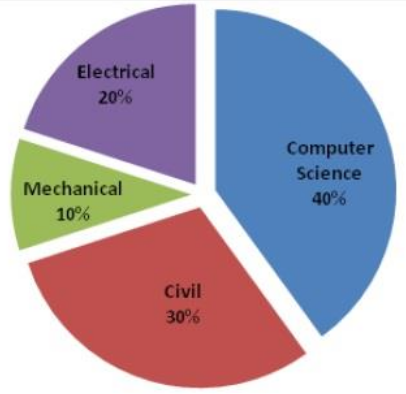
\includegraphics[width=0.5\linewidth]{figs/screenshot001}
	\caption{}
	\label{fig:screenshot001}
\end{figure}
	
		
		\hfill{\brak{\text{GATE CS 2015}}}
		
		\item Select the alternative meaning of the underlined part of the sentence.
		The chain snatchers took to their heels when the police party arrived.
		
		\hfill{\brak{\text{GATE CS 2015}}}
		
		\begin{enumerate}
			\begin{multicols}{2}


			\item took shelter in a thick jungle
			\item open indiscriminate fire
			\item took to flight
			\item unconditionally surrendered 			\end{multicols}
		\end{enumerate}
		
		\item The probabilities that a student passes in Mathematics, Physics and Chemistry are $m$, $p$, and $c$ respectively. Of these subjects, the student has $75\%$ chance of passing in at least one, a $50\%$ chance of passing in at least two and a $40\%$ chance of passing in exactly two. Following relations are drawn in $m$, $p$, $c$:
		\begin{align*}
			\brak{I} \quad p + m + c &= 27/20\\
			\brak{II} \quad p + m + c &= 13/20\\
			\brak{III} \quad \brak{p} \cdot \brak{m} \cdot \brak{c} &= 1/10
		\end{align*}
		
		\hfill{\brak{\text{GATE CS 2015}}}
		
		\begin{enumerate}
			\begin{multicols}{2}
				\item Only relation I is true
				\item Only relation II is true
				\item Relations II and III are true.
				\item Relations I and III are true.
			\end{multicols}
		\end{enumerate}
		
		\item The given statement is followed by some courses of action. Assuming the statement to be true, decide the correct option.
		
		Statement: There has been a significant drop in the water level in the lakes supplying water to the city.
		
		Course of action: I. The water supply authority should impose a partial cut in supply to tackle the situation.
		
		II. The government should appeal to all the residents through mass media for minimal use of water.
		
		III. The government should ban the water supply in lower areas.
		
		\hfill{\brak{\text{GATE CS 2015}}}
		
		\begin{enumerate}
			\begin{multicols}{2}
				\item Statements I and II follow
				\item Statements I and III follow
				\item Statements II and III follow
				\item All statements follow
			\end{multicols}
		\end{enumerate}
		
		\item The number of students in a class who have answered correctly, wrongly, or not attempted each question in an exam, are listed in the table below. The marks for each question are also listed. There is no negative or partial marking.
		
		\begin{table}[h]
			\label{tab:exam_results}
			\begin{center}
				\begin{tabular}{|c|c|c|c|c|}
					\hline
					Q No & Marks & Answered Correctly & Answered Wrongly & Not Attempted \\
					\hline
					$1$ & $2$ & $21$ & $17$ & $6$ \\
					\hline
					$2$ & $3$ & $15$ & $27$ & $2$ \\
					\hline
					$3$ & $1$ & $11$ & $29$ & $4$ \\
					\hline
					$4$ & $2$ & $23$ & $18$ & $3$ \\
					\hline
					$5$ & $5$ & $31$ & $12$ & $1$ \\
					\hline
				\end{tabular}
			\end{center}
		\end{table}
		
		What is the average of the marks obtained by the class in the examination?
		
		\hfill{\brak{\text{GATE CS 2015}}}
		
		\begin{enumerate}
			\begin{multicols}{4}
				\item $2.290$
				\item $2.970$
				\item $6.795$
				\item $8.795$
			\end{multicols}
		\end{enumerate}
		
	\end{enumerate}
	\newpage
	\section*{\Large COMPUTER SCIENCE AND INFORMATION TECHNOLOGY}
	\vspace{0.7cm}
	\fbox{\large Q. No. $1$ - $25$ Carry One Mark Each}
		\vspace{0.7cm}
	\begin{enumerate}
		
		\item Which one of the following is True at any valid state in shift-reduce parsing?
		
		\hfill{\brak{\text{GATE CS 2015}}}
		
		\begin{enumerate}
			\item Viable prefixes appear only at the bottom of the stack and not inside
			\item Viable prefixes appear only at the top of the stack and not inside
			\item The stack contains only a set of viable prefixes
			\item The stack never contains viable prefixes
		\end{enumerate}
		
		\item Match the following:
		
		\begin{table}[h]
			\caption*{}
			\label{tab:match1}
			\begin{center}
				\begin{tabular}{|l|l|}
					\hline
					List - I & List – II \\
					\hline
					\brak{A} Condition coverage & \brak{1} Black-box testing \\
					\hline
					\brak{B} Equivalence class partitioning & \brak{2} System testing \\
					\hline
					\brak{C} Volume testing & \brak{3} White-box testing \\
					\hline
					\brak{D} Alpha testing & \brak{4} Performance testing \\
					\hline
				\end{tabular}
			\end{center}
		\end{table}
		
		\hfill{\brak{\text{GATE CS 2015}}}
		
		\begin{enumerate}
			\begin{multicols}{4}


			\item A $2$ $3$ $1$ $4$
			\item B $3$ $4$ $2$ $1$
			\item C $3$ $1$ $4$ $2$
			\item D $3$ $1$ $2$ $4$
						\end{multicols}
		\end{enumerate}
		
		\item For computers based on three-address instruction formats, each address field can be used to specify which of the following:
		
		S1: A memory operand
		S2: A processor register
		S3: An implied accumulator register
		
		\hfill{\brak{\text{GATE CS 2015}}}
		
		\begin{enumerate}
			\begin{multicols}{2}
				\item Either S1 or S2
				\item Either S2 or S3
				\item Only S2 and S3
				\item All of S1, S2 and S3
			\end{multicols}
		\end{enumerate}
		
		\item Which one of the following is the recurrence equation for the worst case time complexity of the Quicksort algorithm for sorting $n\brak{\geq 2}$ numbers? In the recurrence equations given in the options below, $c$ is a constant.
		
		\hfill{\brak{\text{GATE CS 2015}}}
		
		\begin{enumerate}
			\begin{multicols}{2}
				\item $T\brak{n} = 2T \brak{n/2} + cn$
				\item $T\brak{n} = T\brak{n – 1} + T\brak{1} + cn$
				\item $T\brak{n} = 2T \brak{n – 2} + cn$
				\item $T\brak{n} = T\brak{n/2} + cn$
			\end{multicols}
		\end{enumerate}
		
		\item For any two languages $L_1$ and $L_2$ such that $L_1$ is context free and $L_2$ is recursively enumerable but not recursive, which of the following is/are necessarily true?
		
		I. $\overline{L_1}$ $\brak{complement of L_1}$ is recursive\\
		II. $\overline{L_2}$ $\brak{complement of L_2}$ is recursive\\
		III. $\overline{L_1}$ is context-free\\
		IV. $L_1 \cap L_2$ is recursively enumerable\\
		
		\hfill{\brak{\text{GATE CS 2015}}}
		
		\begin{enumerate}
			\begin{multicols}{4}
				\item I only
				\item III only
				\item III and IV only
				\item I and IV only
			\end{multicols}
		\end{enumerate}
		
		\item Suppose two hosts use a TCP connection to transfer a large file. Which of the following statements is/are FALSE with respect to the TCP connection?
		
		I. If the sequence number of a segment is $m$, then the sequence number of the subsequent segment is always $m+1$.
		
		II. If the estimated round trip time at any given point of time is $t$ sec, the value of the retransmission timeout is always set to greater than or equal to $t$ sec.
		
		III. The size of the advertised window never changes during the course of the TCP connection.
		
		IV. The number of unacknowledged bytes at the sender is always less than or equal to the advertised window
		
		\hfill{\brak{\text{GATE CS 2015}}}
		
		\begin{enumerate}
			\begin{multicols}{4}
				\item III only
				\item I and III only
				\item I and IV only
				\item II and IV only
			\end{multicols}
		\end{enumerate}
		
		\item The following two functions P1 and P2 that share a variable B with an initial value of $2$ execute concurrently.
		
		\begin{align*}
			P1\brak{} \{ \quad &P2\brak{} \{ \\
			C = B – 1; \quad &D = 2 \times B; \\
			B = 2 \times C; \quad &B = D – 1; \\
			\} \quad &\}
		\end{align*}
		
		The number of distinct values that B can possibly take after the execution is \underline{\hspace{2cm}}.
		
		\hfill{\brak{\text{GATE CS 2015}}}
		
		\item Consider a $4$ bit Johnson counter with an initial value of $0000$. The counting sequence of this counter is
		
		\hfill{\brak{\text{GATE CS 2015}}}
		
		\begin{enumerate}
			\begin{multicols}{2}


			\item $0, 1, 3, 7, 15, 14, 12, 8, 0$
			\item $0, 1, 3, 5, 7, 9, 11, 13, 15, 0$
			\item $0, 2, 4, 6, 8, 10, 12, 14, 0$
			\item $0, 8, 12, 14, 15, 7, 3, 1, 0$
						\end{multicols}
		\end{enumerate}
		
		\item Which one of the following fields of an IP header is NOT modified by a typical IP router?
		
		\hfill{\brak{\text{GATE CS 2015}}}
		
		\begin{enumerate}
			\begin{multicols}{2}
				\item Checksum
				\item Source address
				\item Time To Live \brak{TTL}
				\item Length
			\end{multicols}
		\end{enumerate}
		
		\item Select operation in SQL is equivalent to
		
		\hfill{\brak{\text{GATE CS 2015}}}
		
		\begin{enumerate}
			\item the selection operation in relational algebra
			\item the selection operation in relational algebra, except that SELECT in SQL retains duplicates
			\item the projection operation in relational algebra
			\item the projection operation in relational algebra, except that SELECT in SQL retains duplicates
		\end{enumerate}
		
		\item In the LU decomposition of the matrix $\myvec{2 & 2 \\ 4 & 9}$, if the diagonal elements of $U$ are both $1$, then the lower diagonal entry $l_{22}$ of $L$ is \underline{\hspace{2cm}}.
		
		\hfill{\brak{\text{GATE CS 2015}}}
		
		\item Match the following:
		
		\begin{table}[h]
			\caption*{}
			\label{tab:match2}
			\begin{center}
				\begin{tabular}{|l|l|}
					\hline
					List - I & List – II \\
					\hline
					\brak{P} Prim's algorithm for minimum spanning tree & \brak{i} Backtracking \\
					\hline
					\brak{Q} Floyd-Warshall algorithm for all pairs shortest paths & \brak{ii} Greedy method \\
					\hline
					\brak{R} Mergesort & \brak{iii} Dynamic programming \\
					\hline
					\brak{S} Hamiltonian circuit & \brak{iv} Divide and conquer \\
					\hline
				\end{tabular}
			\end{center}
		\end{table}
		
		\hfill{\brak{\text{GATE CS 2015}}}
		
		\begin{enumerate}
			\begin{multicols}{2}


			\item A P iii, Q ii, R iv, S i
			\item B P i, Q ii, R iv, S iii
			\item C P ii, Q iii, R iv, S i
			\item D P ii, Q i, R iii, S iv
						\end{multicols}
		\end{enumerate}
		
		\item The output of the following C program is \underline{\hspace{2cm}}.
		
		\begin{verbatim}
			void f1 (int a, int b)
			{
				int c;
				c=a; a=b; b=c;
			}
			
			void f2 (int *a, int *b)
			{
				int c;
				c=*a; *a=*b;*b=c;
			}
			
			int main( )
			{
				int a=4, b=5, c=6;
				f1 (a, b);
				f2 (&b, &c);
				printf ("%d", c-a-b);
			}
		\end{verbatim}
		
		\hfill{\brak{\text{GATE CS 2015}}}
		
		\item $\lim_{x \to 1} \frac{x}{x}$ is \underline{\hspace{2cm}}
		
		\hfill{\brak{\text{GATE CS 2015}}}
		
		\begin{enumerate}
			\begin{multicols}{4}
				\item $\infty$
				\item $0$
				\item $1$
				\item Not defined
			\end{multicols}
		\end{enumerate}
		
		\item For a set $A$, the power set of $A$ is denoted by $2^A$. If $A = \{5, \{6\}, \{7\}\}$, which of the following options are True?
		
		$1.$ $\emptyset \in 2^A$
		$2.$ $\{5\} \in 2^A$
		$3.$ $\{\{5, 6\}\} \in 2^A$
		$4.$ $\{5, 6\} \in 2^A$
		
		\hfill{\brak{\text{GATE CS 2015}}}
		
		\begin{enumerate}
			\begin{multicols}{4}
				\item $1$ and $3$ only
				\item $2$ and $3$ only
				\item $1, 2$ and $3$ only
				\item $1, 2$ and $4$ only
			\end{multicols}
		\end{enumerate}
		
		\item Consider a system with byte-addressable memory, $32$ bit logical addresses, $4$ kilobyte page size and page table entries of $4$ bytes each. The size of the page table in the system in megabytes is \underline{\hspace{2cm}}.
		
		\hfill{\brak{\text{GATE CS 2015}}}
		
		\item A file is organized so that the ordering of data records is the same as or close to the ordering of data entries in some index. Then that index is called
		
		\hfill{\brak{\text{GATE CS 2015}}}
		
		\begin{enumerate}
			\begin{multicols}{4}
				\item Dense
				\item Sparse
				\item Clustered
				\item Unclustered
			\end{multicols}
		\end{enumerate}
		
		\item What are the worst-case complexities of insertion and deletion of a key in a binary search tree?
		
		\hfill{\brak{\text{GATE CS 2015}}}
		
		\begin{enumerate}
			\item $\theta\brak{\log n}$ for both insertion and deletion
			\item $\theta\brak{n}$ for both insertion and deletion
			\item $\theta\brak{n}$ for insertion and $\theta\brak{\log n}$ for deletion
			\item $\theta\brak{\log n}$ for insertion and $\theta\brak{n}$ for deletion
		\end{enumerate}
		
		\item Suppose that everyone in a group of $N$ people wants to communicate secretly with the $N–1$ others using symmetric key cryptographic system. The communication between any two persons should not be decodable by the others in the group. The number of keys required in the system as a whole to satisfy the confidentiality requirement is
		
		\hfill{\brak{\text{GATE CS 2015}}}
		
		\begin{enumerate}
			\begin{multicols}{4}
				\item $2N$
				\item $N\brak{N – 1}$
				\item $N\brak{N – 1}/2$
				\item $\brak{N – 1}^2$
			\end{multicols}
		\end{enumerate}
		
		\item Which one of the following is Not equivalent to $p \leftrightarrow q$?
		
		\hfill{\brak{\text{GATE CS 2015}}}
		
		\begin{enumerate} 			\begin{multicols}{4}
			\item $\brak{\neg p \lor q} \land \brak{p \lor \neg q}$
			\item $\brak{\neg p \lor q} \land \brak{q \to p}$
			\item $\brak{\neg p \lor q} \land \brak{p \lor \neg q}$
			\item $\brak{\neg p \lor \neg q} \land \brak{p \lor q}$ 			\end{multicols}
		\end{enumerate}
		
		\item Which of the following is/are correct inorder traversal sequence\brak{s} of binary search tree\brak{s}?
		
		$1.$ $3, 5, 7, 8, 15, 19, 25$
		$2.$ $5, 8, 9, 12, 10, 15, 25$
		$3.$ $2, 7, 10, 8, 14, 16, 20$
		$4.$ $4, 6, 7, 9, 18, 20, 25$
		
		\hfill{\brak{\text{GATE CS 2015}}}
		
		\begin{enumerate}
			\begin{multicols}{4}
				\item $1$ and $4$ only
				\item $2$ and $3$ only
				\item $2$ and $4$ only
				\item $2$ only
			\end{multicols}
		\end{enumerate}
		
		\item In one of the pairs of protocols given below, both the protocols can use multiple TCP connections between the same client and the server. Which one is that?
		
		\hfill{\brak{\text{GATE CS 2015}}}
		
		\begin{enumerate}
			\begin{multicols}{4}
				\item HTTP, FTP
				\item HTTP, TELNET
				\item FTP, SMTP
				\item HTTP, SMTP
			\end{multicols}
		\end{enumerate}
		
		\item Which of following statements is/are FALSE?
		
		I. XML overcomes the limitations in HTML to support a structured way of organizing content.
		II. XML specification is not case sensitive while HTML specification is case sensitive.
		III. XML supports user defined tags while HTML uses pre-defined tags.
		VI. XML tags need not be closed while HTML tags must be closed
		
		\hfill{\brak{\text{GATE CS 2015}}}
		
		\begin{enumerate}
			\begin{multicols}{4}
				\item II only
				\item I only
				\item II and IV only
				\item III and IV only
			\end{multicols}
		\end{enumerate}
		
		\item If $g\brak{x} = 1 – x$ and h(x) = $\frac{x}{x - 1}$ then $\frac{g(h(x))}{h(g(x))}$ is
		
		\hfill{\brak{\text{GATE CS 2015}}}
		
		\begin{enumerate}			\begin{multicols}{4}
			\item $\frac{h\brak{x}}{g\brak{x}}$
			\item - $\frac{1}{x}$
			\item $\frac{g\brak{x}}{h\brak{x}}$
			\item $\frac{x}{(1-x)^2}$ 			\end{multicols}
		\end{enumerate}
		
		\item The height of a tree is the length of the longest root-to-leaf path in it. The maximum and minimum number of nodes in a binary tree of height $5$ are
		
		\hfill{\brak{\text{GATE CS 2015}}}
		
		\begin{enumerate}
			\begin{multicols}{2}
				\item $63$ and $6$, respectively
				\item $64$ and $5$, respectively
				\item $32$ and $6$, respectively
				\item $31$ and $5$, respectively
			\end{multicols}
		\end{enumerate}
		
	\end{enumerate}
	
	\fbox{\large Q. No. $26$-$55$ Carry Two Marks Each}
	
	\begin{enumerate}[resume]
		
		\item What is the output of the following C code?
		Assume that the address of X is $2000$ \brak{in decimal} and an integer requires four bytes of memory.
		
		\begin{verbatim}
			int main()
			{
				unsigned int x[4][3] = {{1,2,3},{4,5,6},{7,8,9},{10,11,12}};
				printf("%u,%u,%u", x+3, *(x+3), *(x+2)+3);
			}
		\end{verbatim}
		
		\hfill{\brak{\text{GATE CS 2015}}}
		
		\begin{enumerate}
			\begin{multicols}{2}
				\item $2036, 2036, 2036$
				\item $2012,4,2204$
				\item $2036,10,10$
				\item $2012,4,6$
			\end{multicols}
		\end{enumerate}
		
		\item Consider the DFAs M and N given above. The number of states in a minimal DFA that accepts the language $L\brak{M} \cap L\brak{N}$ is \underline{\hspace{2cm}}.
		
		\begin{figure}[H]
			\centering
			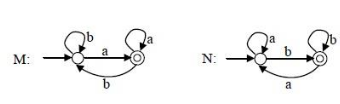
\includegraphics[width=0.5\linewidth]{figs/screenshot002}
		\end{figure}
		
		
		\hfill{\brak{\text{GATE CS 2015}}}
		
		\item Consider a non-pipelined processor with a clock rate of $2.5$ gigahertz and average cycles per instruction of four. The same processor is upgraded to a pipelined processor with five stages; but due to the internal pipeline delay, the clock speed is reduced to $2$ gigahertz. Assume that there are no stalls in the pipeline. The speed up achieved in this pipelined processor is \underline{\hspace{2cm}}.
		
		\hfill{\brak{\text{GATE CS 2015}}}
		
		\item The least number of temporary variables required to create a three-address code in static single assignment form for the expression $q + r/3 + s – t \times 5 + u \times v/w$ is \underline{\hspace{2cm}}.
		
		\hfill{\brak{\text{GATE CS 2015}}}
		
		\item Suppose $L = \{p, q, r, s, t\}$ is a lattice represented by the following Hasse diagram:
		
		\begin{figure}[H]
			\centering
			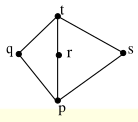
\includegraphics[width=0.3\linewidth]{figs/screenshot003}
			\caption{}
			\label{fig:screenshot003}
		\end{figure}
		
		
		For any $x,y \in L$, not necessarily distinct, $x \lor y$ and $x \land y$ are join and meet of $x, y$ respectively. Let $L^3 = \{\brak{x,y,z}\colon x, y, z \in L\}$ be the set of all ordered triplets of the elements of $L$. Let Pr be the probability that an element $\brak{x,y,z} \in L^3$ chosen equiprobably satisfies $x \lor \brak{y \land z} = \brak{x \lor y} \land \brak{x \lor z}$. Then
		
		\hfill{\brak{\text{GATE CS 2015}}}
		
		\begin{enumerate}
			\begin{multicols}{4}
				\item Pr $= 0$
				\item Pr $= 1$
				\item $0 <$ Pr $\leq 1/5$
				\item $1/5 <$ Pr $< 1$
			\end{multicols}
		\end{enumerate}
		
		\item Consider the NPDA $<Q = \{q_0, q_1, q_2\}, \Sigma = \{0, 1\}, \Gamma = \{0, 1, Z_0\}, \delta, q_0, Z_0, F = \{q_2\}>$, where \brak{as per usual convention} $Q$ is the set of states, $\Sigma$ is the input alphabet, $\Gamma$ is stack alphabet, $\delta$ is the state transition function, $q_0$ is the initial state, $Z_0$ is the initial stack symbol, and $F$ is the set of accepting states, The state transition is as follows
		
		\begin{figure}[H]
			\centering
			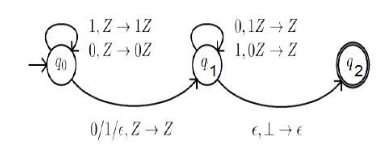
\includegraphics[width=0.5\linewidth]{figs/screenshot004}
			\caption{}
			\label{fig:screenshot004}
		\end{figure}
		
		
		Which one of the following sequences must follow the string $101100$ so that the overall string is accepted by the automaton?
		
		\hfill{\brak{\text{GATE CS 2015}}}
		
		\begin{enumerate}
			\begin{multicols}{4}
				\item $10110$
				\item $10010$
				\item $01010$
				\item $01001$
			\end{multicols}
		\end{enumerate}
		
		\item Consider the following pseudo code, where $x$ and $y$ are positive integers.
		
		\begin{align*}
			&\text{begin}\\
			&q := 0\\
			&r := x\\
			&\text{while } r \geq y \text{ do}\\
			&\quad \text{begin}\\
			&\quad\quad r := r – y\\
			&\quad\quad q := q + 1\\
			&\quad \text{end}\\
			&\text{end}
		\end{align*}
		
		The post condition that needs to be satisfied after the program terminates is
		
		\hfill{\brak{\text{GATE CS 2015}}}
		
		\begin{enumerate}
						\begin{multicols}{2}
			\item $\{r = qx+ y \land r <y\}$
			\item $\{x = qy+ r \land r<y\}$
			\item $\{y = qx+ r \land 0 <r <y\}$
			\item $\{q + 1 <r – y \land y> 0\}$ 			\end{multicols}
		\end{enumerate}
		
		\item An algorithm performs $\brak{\log N}^{1/2}$ find operations, $N$ insert operations, $\brak{\log N}^{1/2}$ delete operations, and $\brak{\log N}^{1/2}$ decrease-key operations on a set of data items with keys drawn from a linearly ordered set. For a delete operation, a pointer is provided to the record that must be deleted.
		
		For the decrease-key operation, a pointer is provided to the record that has its key decreased. Which one of the following data structures is the most suited for the algorithm to use, if the goal is to achieve the best total asymptotic complexity considering all the operations?
		
		\hfill{\brak{\text{GATE CS 2015}}}
		
		\begin{enumerate}
			\begin{multicols}{2}
				\item Unsorted array
				\item Min-heap
				\item Sorted array
				\item Sorted doubly linked list
			\end{multicols}
		\end{enumerate}
		
		\item Consider a max heap, represented by the array: $40, 30, 20, 10, 15, 16, 17, 8, 4$.
		
		\begin{table}[h]
			\caption*{}
			\label{tab:heap_array}
			\begin{center}
				\begin{tabular}{|c|c|c|c|c|c|c|c|c|c|}
					\hline
					Array Index & $1$ & $2$ & $3$ & $4$ & $5$ & $6$ & $7$ & $8$ & $9$ \\
					\hline
					Value & $40$ & $30$ & $20$ & $10$ & $15$ & $16$ & $17$ & $8$ &$4$ \\
					\hline
				\end{tabular}
			\end{center}
		\end{table}
		
		Now consider that a value $35$ is inserted into this heap. After insertion, the new heap is
		
		\hfill{\brak{\text{GATE CS 2015}}}
		
		\begin{enumerate}
						\begin{multicols}{2}
			\item $40, 30, 20, 10, 15, 16, 17, 8, 4, 35$
			\item $40, 35, 20, 10, 30, 16, 17, 8, 4, 15$
			\item $40, 30, 20, 10, 35, 16, 17, 8, 4, 15$
			\item $40, 35, 20, 10, 15, 16, 17, 8, 4, 30$ 			\end{multicols}
		\end{enumerate}
		
		\item Consider the following $2 \times 2$ matrix $A$ where two elements are unknown and are marked by $a$ and $b$. The eigenvalues of this matrix are $-1$ and $7$. What are the values of $a$ and $b$?
		
		$A = \myvec{1 & 4 \\ b & a}$
		
		\hfill{\brak{\text{GATE CS 2015}}}
		
		\begin{enumerate}
									\begin{multicols}{2}
			\item $a = 6, b = 4$
			\item $a = 4, b = 6$
			\item $a = 3, b = 5$
			\item $a = 5, b = 3$ \end{multicols}
		\end{enumerate}
		
		\item Let $G = \brak{V, E}$ be a simple undirected graph, and $s$ be a particular vertex in it called the source. For $x \in V$, let $d\brak{x}$ denote the shortest distance in $G$ from $s$ to $x$. A breadth first search \brak{BFS} is performed starting at $s$. Let $T$ be the resultant BFS tree. If $\brak{u, v}$ is an edge of $G$ that is not in $T$, then which one of the following CANNOT be the value of $d\brak{u} – d\brak{v}$?
		
		\hfill{\brak{\text{GATE CS 2015}}}
		
		\begin{enumerate}
			\begin{multicols}{4}
				\item $–1$
				\item $0$
				\item $1$
				\item $2$
			\end{multicols}
		\end{enumerate}
		
		\item The binary operator $\oplus$ is defined by the following truth table:
		
		\begin{table}[h]
			\caption*{}
			\label{tab:truth_table}
			\begin{center}
				\begin{tabular}{|c|c|c|}
					\hline
					$p$ & $q$ & $p \oplus q$ \\
					\hline
					$0$ & $0$ & $0$ \\
					$0$ & $1$ & $1$ \\
					$1$ & $0$ & $1$ \\
					$1$ & $1$ & $0$ \\
					\hline
				\end{tabular}
			\end{center}
		\end{table}
		
		Which one of the following is true about the binary operator $\oplus$?
		
		\hfill{\brak{\text{GATE CS 2015}}}
		
		\begin{enumerate}
			\begin{multicols}{2}


			\item Both commutative and associative
			\item Commutative but not associative
			\item Not commutative but associative
			\item Neither commutative nor associative
						\end{multicols}
		\end{enumerate}
		
		\item Consider an Entity-Relationship \brak{ER} model in which entity sets $E_1$ and $E_2$ are connected by an $m:n$ relationship $R_{12}$, $E_1$ and $E_3$ are connected by a $1 \colon n$ $\brak{1 on the side of E_1 and n on the side of E_3}$ relationship $R_{13}$.
		
		$E_1$ has two single-valued attributes $a_{11}$ and $a_{12}$ of which $a_{11}$ is the key attribute. $E_2$ has two single-valued attributes $a_{21}$ and $a_{22}$ of which $a_{21}$ is the key attribute. $E_3$ has two single-valued attributes $a_{31}$ and $a_{32}$ of which $a_{31}$ is the key attribute. The relationships do not have any attributes.
		
		If a relational model is derived from the above ER model, then the minimum number of relations that would be generated if all the relations are in 3NF is \underline{\hspace{2cm}}.
		
		\hfill{\brak{\text{GATE CS 2015}}}
		
		\item The graph shown below $8$ edges with distinct integer edge weights. The minimum spanning tree \brak{MST} is of weight $36$ and contains the edges: $\{\brak{A, C}, \brak{B, C}, \brak{B, E}, \brak{E, F}, \brak{D, F}\}$. The edge weights of only those edges which are in the MST are given in the figure shown below.
		
	\begin{figure}[H]
		\centering
		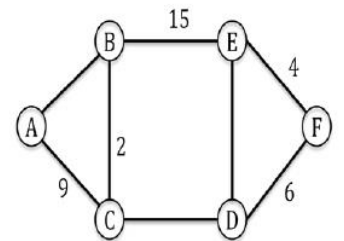
\includegraphics[width=0.3\linewidth]{figs/screenshot005}
		\caption{}
		\label{fig:screenshot005}
	\end{figure}
	
		
		The minimum possible sum of weights of all $8$ edges of this graph is \underline{\hspace{2cm}}.
		
		\hfill{\brak{\text{GATE CS 2015}}}
		
		\item Consider a disk pack with a seek time of $4$ milliseconds and rotational speed of $10000$ rotations per minute \brak{RPM}. It has $600$ sectors per track and each sector can store $512$ bytes of data. Consider a file stored in the disk. The file contains $2000$ sectors. Assume that every sector access necessitates a seek, and the average rotational latency for accessing each sector is half of the time for one complete rotation. The total time \brak{in milliseconds} needed to read the entire file is \underline{\hspace{2cm}}.
		
		\hfill{\brak{\text{GATE CS 2015}}}
		
		\item $\int_{\frac{1}{\pi}}^{\frac{2}{\pi}} \frac{\cos(\frac{1}{x})}{x^2} dx$ is \underline{\hspace{2cm}}.
		
		\hfill{\brak{\text{GATE CS 2015}}}
		
		\item Consider the following C program segment.
		
		\begin{verbatim}
			while (first <= last)
			{
				if (array [middle] < search)
				first = middle +1;
				else if (array [middle] == search)
				found = True;
				else last = middle – 1;
				middle = (first + last)/2;
			}
			if (first > last) notPresent = True;
		\end{verbatim}
		
		The cyclomatic complexity of the program segment is \underline{\hspace{2cm}}.
		
		\hfill{\brak{\text{GATE CS 2015}}}
		
		\item Consider the following C function.
		
		\begin{verbatim}
			int fun1 (int n)
			{
				int i, j, k, p, q = 0;
				for (i = 1; i<n; ++i)
				{
					p = 0;
					for (j=n; j>1; j=j/2)
					++p;
					for (k=1; k<p; k=k*2)
					++q;
				}
				return q;
			}
		\end{verbatim}
		
		Which one of the following most closely approximates the return value of the function fun1?
		
		\hfill{\brak{\text{GATE CS 2015}}}
		
		\begin{enumerate}
			\begin{multicols}{4}
				\item $n^3$
				\item $n\brak{\log n}^2$
				\item $n\log n$
				\item $n\log\brak{\log n}$
			\end{multicols}
		\end{enumerate}
		
		\item Let $a_n$ represent the number of bit strings of length $n$ containing two consecutive $1$s. What is the recurrence relation for $a_n$?
		
		\hfill{\brak{\text{GATE CS 2015}}}
		
		\begin{enumerate}
						\begin{multicols}{2}
			\item $a_{n–2} + a_{n–1} + 2^{n–2}$
			\item $a_{n–2} + 2a_{n–1} + 2^{n–2}$
			\item $2a_{n–2} + a_{n–1} + 2^{n–2}$
			\item $2a_{n–2} + 2a_{n–1} + 2^{n–2}$ 			\end{multicols}
		\end{enumerate}
		
		\item A variable $x$ is said to be live at a statement $S_i$ in a program if the following three conditions hold simultaneously:\\
		$1.$ There exists a statement $S_j$ that uses $x$\\
		$2.$ There is a path from $S_i$ to $S_j$ in the flow graph corresponding to the program\\
		$3.$ The path has no intervening assignment to $x$ including at $S_i$ and $S_j$\\
		
		\begin{figure}[H]
			\centering
			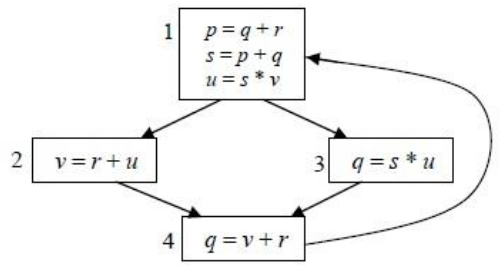
\includegraphics[width=0.5\linewidth]{figs/screenshot006}
			\caption{}
			\label{fig:screenshot006}
		\end{figure}
		
		
		The variables which are live both at the statement in basic block $2$ and at the statement in basic block $3$ of the above control flow graph are
		
		\hfill{\brak{\text{GATE CS 2015}}}
		
		\begin{enumerate}
			\begin{multicols}{4}
				\item $p, s, u$
				\item $r, s, u$
				\item $r, u$
				\item $q, v$
			\end{multicols}
		\end{enumerate}
		
		\item Consider a uniprocessor system executing three tasks $T_1$, $T_2$ and $T_3$, each of which is composed of an infinite sequence of jobs \brak{or instances} which arrive periodically at intervals of $3$, $7$ and $20$ milliseconds, respectively. The priority of each task is the inverse of its period and the available tasks are scheduled in order of priority, with the highest priority task scheduled first. Each instance of $T_1$, $T_2$ and $T_3$ requires an execution time of $1$, $2$ and $4$ milliseconds, respectively. Given that all tasks initially arrive at the beginning of the $1$st millisecond and task preemptions are allowed, the first instance of $T_3$ completes its execution at the end of \underline{\hspace{2cm}} milliseconds.
		
		\hfill{\brak{\text{GATE CS 2015}}}
		
		\item Consider the following relations:
		
		\begin{table}[h]
			\caption*{}
			\label{tab:student_performance}
			\begin{center}
				\begin{tabular}{|c|c|}
					\hline
					\multicolumn{2}{|c|}{Student:} \\
					\hline
					Roll No & Student Name \\
					\hline
					$1$ & Raj \\
					\hline
					$2$ & Rohit \\
					\hline
					$3$ & Raj \\
					\hline
				\end{tabular}
				\quad
				\begin{tabular}{|c|c|c|}
					\hline
					\multicolumn{3}{|c|}{Performance:} \\
					\hline
					Roll No & Course & Marks \\
					\hline
					$1$ & Math & $80$ \\
					\hline
					$1$ & English & $70$ \\
					\hline
					$2$ & Math & $75$ \\
					\hline
					$3$ & English & $80$ \\
					\hline
					$2$ & Physics & $65$ \\
					\hline
					$3$ & Math & $80$ \\
					\hline
				\end{tabular}
			\end{center}
		\end{table}
		
		Consider the following SQL query.
		\begin{verbatim}
			SELECT S.Student_Name, sum (P.Marks)
			FROM Student S, Performance P
			WHERE S.Roll_No = P.Roll_No
			GROUP BY S.Student_Name
		\end{verbatim}
		
		The number of rows that will be returned by the SQL query is \underline{\hspace{2cm}}.
		
		\hfill{\brak{\text{GATE CS 2015}}}
		
		\item A positive edge-triggered D flip-flop is connected to a positive edge-triggered JK flipflop as follows. The Q output of the D flip-flop is connected to both the J and K inputs of the JK flip-flop, while the Q output of the JK flip-flop is connected to the input of the D flip-flop. Initially, the output of the D flip-flop is set to logic one and the output of the JK flip-flop is cleared. Which one of the following is the bit sequence \brak{including the initial state} generated at the Q output of the JK flip-flop when the flip-flops are connected to a free-running common clock? Assume that $J = K = 1$ is the toggle mode and $J = K = 0$ is the state-holding mode of the JK flip-flop. Both the flip-flops have non-zero propagation delays.
		
		\hfill{\brak{\text{GATE CS 2015}}}
		
		\begin{enumerate}
			\begin{multicols}{4}


			\item $0110110...$
			\item $0100100...$
			\item $011101110...$
			\item $011001100...$
						\end{multicols}
		\end{enumerate}
		
		\item Let $G$ be a connected planar graph with $10$ vertices. If the number of edges on each face is three, then the number of edges in $G$ is \underline{\hspace{2cm}}.
		
		\hfill{\brak{\text{GATE CS 2015}}}
		
		\item Consider a LAN with four nodes $S_1$, $S_2$, $S_3$ and $S_4$. Time is divided into fixed-size slots, and a node can begin its transmission only at the beginning of a slot. A collision is said to have occurred if more than one node transmit in the same slot. The probabilities of generation of a frame in a time slot by $S_1$, $S_2$, $S_3$ and $S_4$ are $0.1$, $0.2$, $0.3$ and $0.4$, respectively. The probability of sending a frame in the first slot without any collision by any of these four stations is \underline{\hspace{2cm}}.
		
		\hfill{\brak{\text{GATE CS 2015}}}
		
		\item Suppose the following disk request sequence \brak{track numbers} for a disk with $100$ tracks is given: $45, 20, 90, 10, 50, 60, 80, 25, 70$. Assume that the initial position of the R/W head is on track $50$. The additional distance that will be traversed by the R/W head when the Shortest Seek Time First \brak{SSTF} algorithm is used compared to the SCAN \brak{Elevator} algorithm (assuming that SCAN algorithm moves towards 100 when it starts execution) is \underline{\hspace{2cm}} tracks.
		
		\hfill{\brak{\text{GATE CS 2015}}}
		
		\item Suppose that the stop-and-wait protocol is used on a link with a bit rate of $64$ kilobits per second and $20$ milliseconds propagation delay. Assume that the transmission time for the acknowledgment and the processing time at nodes are negligible. Then the minimum frame size in bytes to achieve a link utilization of at least $50\%$ is \underline{\hspace{2cm}}.
		
		\hfill{\brak{\text{GATE CS 2015}}}
		
		\item Consider a main memory with five page frames and the following sequence of page references: $3, 8, 2, 3, 9, 1, 6, 3, 8, 9, 3, 6, 2, 1, 3$. Which one of the following is true with respect to page replacement policies First-In-First Out \brak{FIFO} and Least Recently Used \brak{LRU}?
		
		\hfill{\brak{\text{GATE CS 2015}}}
		
		\begin{enumerate}
						\begin{multicols}{2}
			\item Both incur the same number of page faults
			\item FIFO incurs $2$ more page faults than LRU
			\item LRU incurs $2$ more page faults than FIFO
			\item FIFO incurs $1$ more page faults than LRU 						\end{multicols}
			
		\end{enumerate}
		
		\item Consider the operations
		\begin{align*}
			f \brak{X,Y,Z } &= X'YZ + XY' + Y'Z'\\
			g \brak{X,Y,Z } &= X'YZ + X'YZ' + XY
		\end{align*}
		
		Which one of the following is CORRECT?
		
		\hfill{\brak{\text{GATE CS 2015}}}
		
		\begin{enumerate}
									\begin{multicols}{2}
			\item Both $\{f\}$ and $\{g\}$ are functionally complete
			\item Only $\{f\}$ is functionally complete
			\item Only $\{g\}$ is functionally complete
			\item Neither $\{f\}$ nor $\{g\}$ is functionally complete
		\end{multicols}
		\end{enumerate}
		
		\item $\sum_{x=1}^{99} \frac{1}{x\brak{x+1}}$ is \underline{\hspace{2cm}}.
		
		\hfill{\brak{\text{GATE CS 2015}}}
		
	\end{enumerate}
	
\end{document}
